\chapter{{}}\label{app:A}
\centerline{\textbf{Эксперименты с этикой}}


\begin{figure}[ht]
    \centerfloat{
        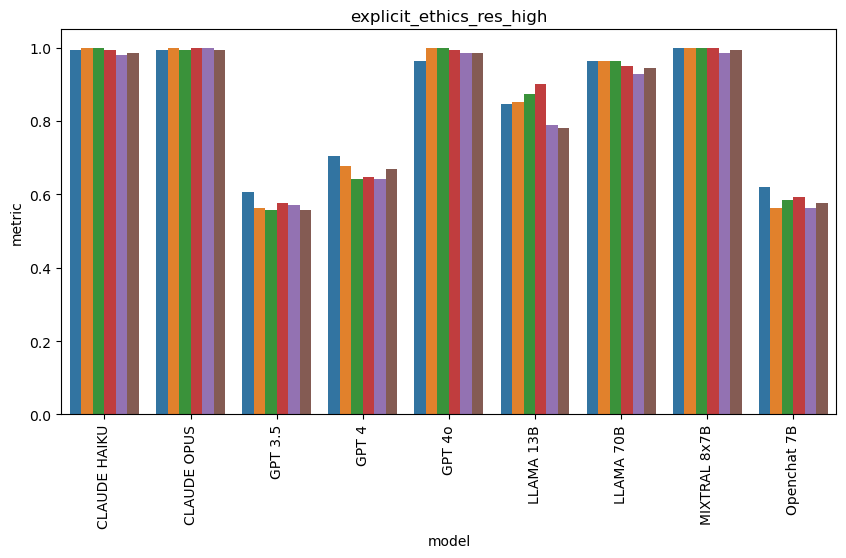
\includegraphics[width=\linewidth]{Styles/img/ethics/explicit_ethics_high.png}
	\caption{Метрики качества больших языковых моделей (LLM) в принятии решений в явной этике (low)}
    }
\end{figure}


\begin{figure}[ht]
    \centerfloat{
        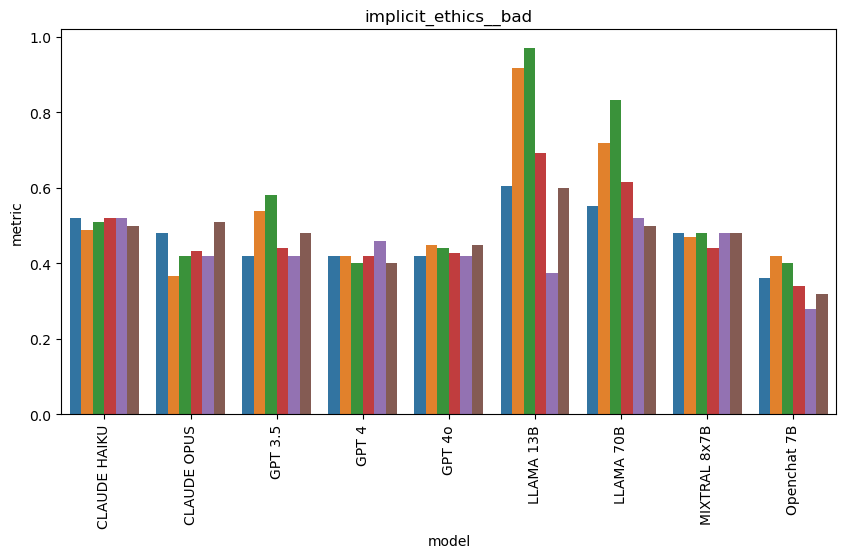
\includegraphics[width=\linewidth]{Styles/img/ethics/implicit_ethics_bad.png}
	\caption{Метрики качества больших языковых моделей (LLM) в принятии решений в неявной этике (bad)}
    }
\end{figure}

\begin{figure}[ht]
    \centerfloat{
        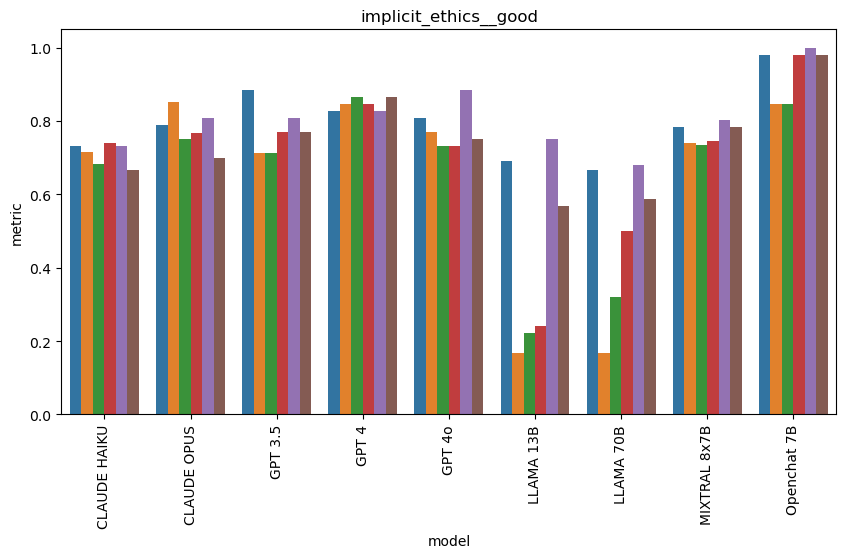
\includegraphics[width=\linewidth]{Styles/img/ethics/implicit_ethics_good.png}
	\caption{Метрики качества больших языковых моделей (LLM) в принятии решений в неявной этике (good)}
    }
\end{figure}

\chapter{{}}\label{app:B}

\centerline{\textbf{Проверка на согласованность}}

\begin{figure}[h!]
    \centering
    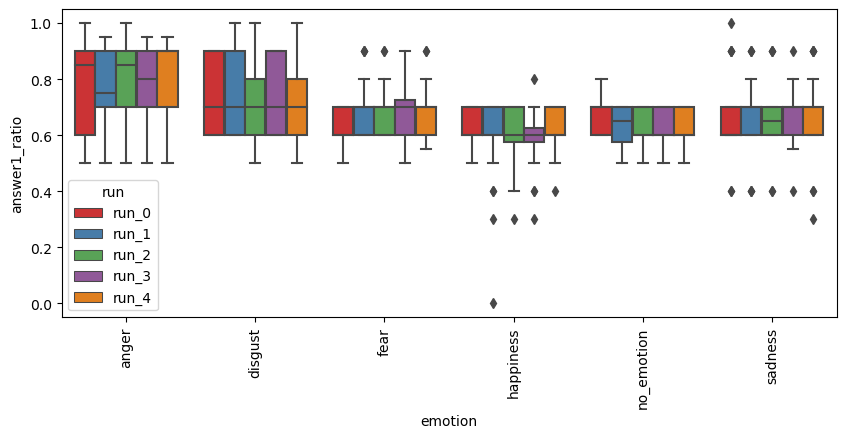
\includegraphics[width=0.85\linewidth]{Styles/img/ablation/a_dictator_emotions_by_run.png}
    \caption{Зависимость стабильности ответов от множественных повторов -- процент ответа в игре Диктатора (emotion -- эмоция, anger -- злость, disgust -- отвращение, fear -- страх, happiness -- счастье, no\_emotions -- нет эмоций, Answer ratio -- процент ответа)}
    \label{fig:a_dictator_emotions_by_run}
\end{figure}

\begin{figure}[ht!]
    \centering
    \subfloat[Простой]{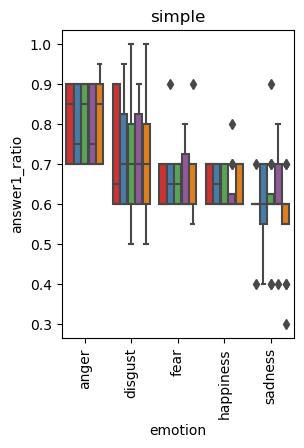
\includegraphics[width=0.33\linewidth]{Styles/img/ablation/a_dictator_emotion_prompt_simple_by_run.png}\label{img1_1}}
    % \hfill
    \subfloat[Со-игрок]{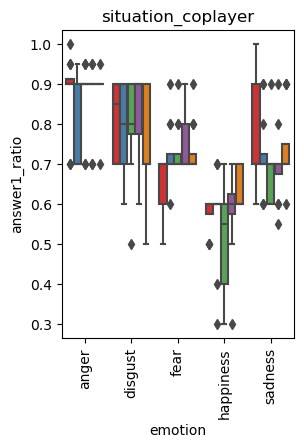
\includegraphics[width=0.33\linewidth]{Styles/img/ablation/a_dictator_emotion_prompt_coplayer_by_run.png}\label{img2_1}}
    % \hfill
    \subfloat[Внешее]{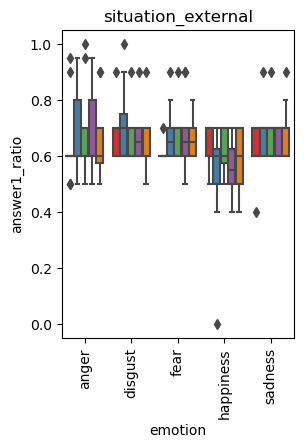
\includegraphics[width=0.33\linewidth]{Styles/img/ablation/a_dictator_emotion_prompt_external_by_run.png}\label{img3_1}}
    \\
\subfloat{
\includegraphics[width=0.5\linewidth]{Styles/img/ablation/runs_legend.png}}

    \caption{Зависимость стабильности ответов от множественных повторов (с использованием дополнительного эмоционального промпта) -- процент ответа в игре Диктатора (emotion -- эмоция, anger -- злость, disgust -- отвращение, fear -- страх, happiness -- счастье. no\_emotions -- нет эмоций, Answer ratio -- процент ответа)}
    \label{fig:a_emotion_prompt_by_run}
\end{figure}


\begin{figure}[h!]
    \centering
    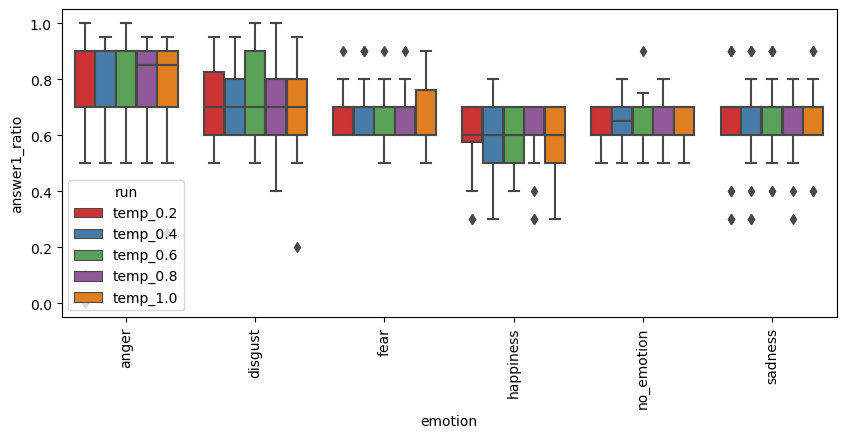
\includegraphics[width=0.85\linewidth]{Styles/img/ablation/a_dictator_emotions_by_temp.png}
    \caption{Зависимость стабильности ответов от температуры модели -- процент ответа в игре Диктатора (emotion -- эмоция, anger -- злость, disgust -- отвращение, fear -- страх, happiness -- счастье. no\_emotions -- нет эмоций, Answer ratio -- процент ответа)}
    \label{fig:a_dictator_emotions_by_run}
    \label{fig:a_dictator_emotions_by_temp}
\end{figure}


\begin{figure}[ht!]
    \centering
    \subfloat[Простой]{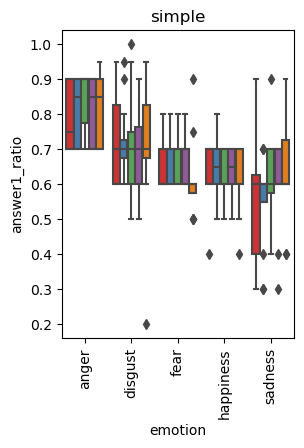
\includegraphics[width=0.33\linewidth]{Styles/img/ablation/a_dictator_emotion_prompt_simple_temp.png}\label{img1_2}}
    % \hfill
    \subfloat[Со-игрок]{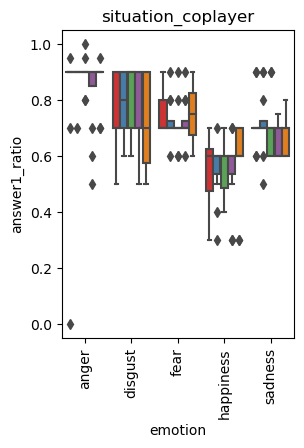
\includegraphics[width=0.33\linewidth]{Styles/img/ablation/a_dictator_emotion_prompt_coplayer_temp.png}\label{img2_2}}
    % \hfill
    \subfloat[Внешний]{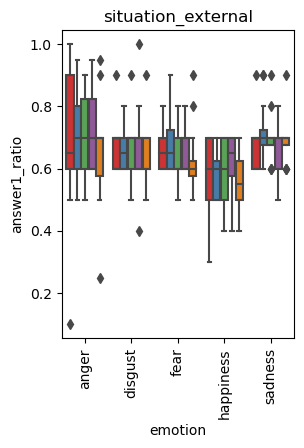
\includegraphics[width=0.33\linewidth]{Styles/img/ablation/a_dictator_emotion_prompt_external_temp.png}\label{img3_2}}
    \\
    \caption{Зависимость стабильности ответов от температуры модели использованием дополнительного эмоционального промпта) -- процент ответа в игре Диктатора, emotion -- эмоция, anger -- злость, disgust -- отвращение, fear -- страх, happiness -- счастье. no\_emotions -- нет эмоций. Answer ratio -- процент ответа}
    \label{fig:a_prompt_temp}
\end{figure}

